Fig.\ref{fig:v} upper panel Shows the cross correlation between 
the reconstructed velocity field $\hat v_{z,ns}$ and the real velocity field $v_z$, at redshift 1 and 2. 

At this point, all the manipulation and calculation on $\delta(\bm{k})$ are independent over different $\bm{k}$, 
therefore, the cross-correlation closely resembles the substraction we perform. 

Just one interesting thing to notice is that although the foreground at z=2 is stronger, 
the non-linear effects are weaker.  
So we still can obtain correlations at $k_\parallel \lesssim 0.1$ with the seriously suppressed density contrast. 

Fig.\ref{fig:r} shows the cross correlation between the reconstructed kSZ map 
$\hat\Theta_{ns}$ and real kSZ map $\Theta$ at redshift 1 and 2. 

There are two points to notice: 

(1) For both redshift, there are a considerable amount of correlation 
$r\gtrsim0.5$ for $l\gtrsim 1000$; 
and this correlation drops quickly for smalller$\ell$; 

(2) The obtained correlation at redshift 2 is better than redshift 1.

Although not satisfactory at small$\ell$, the reconstructed kSZ signal $\hat \Theta_{ns}$ 
from 21cm density field shall already be able to give us reasonable S/N in real applications  
, because most kSZ signals that can actually be distinguished come from at least $l\gtrsim 500$, when primary CMB gradually dies out. 

%However, based on the analysis above, 
%we will expect a further improvement on cross correlation 
%if we recover the small k modes lost in noises. 
%In next section, we provide a method to achieve the goal.


\begin{figure}[tbp]
\begin{center}
\includegraphics[width=0.48\textwidth]{compare_powv2d_z1z2.eps}
\end{center}
\vspace{-0.7cm}
\caption{(Top) The cross correlation r between $P_{v_z}$ and 
    $P_{\hat v_z^{fs}}$ calculated from foreground substracted field $\delta_{fs}$; 
    (Bottom) The cross correlation between $P_{v_z}$ and $P_{\hat v_z^{tide}}$ calculated from $\hat \kappa_c$. 
%The contour line indicates $k^3 P(k)$.
}
\label{fig:v}
\end{figure}
